\documentclass{beamer}\usepackage[]{graphicx}\usepackage[]{color}
% maxwidth is the original width if it is less than linewidth
% otherwise use linewidth (to make sure the graphics do not exceed the margin)
\makeatletter
\def\maxwidth{ %
  \ifdim\Gin@nat@width>\linewidth
    \linewidth
  \else
    \Gin@nat@width
  \fi
}
\makeatother

\definecolor{fgcolor}{rgb}{0.345, 0.345, 0.345}
\newcommand{\hlnum}[1]{\textcolor[rgb]{0.686,0.059,0.569}{#1}}%
\newcommand{\hlstr}[1]{\textcolor[rgb]{0.192,0.494,0.8}{#1}}%
\newcommand{\hlcom}[1]{\textcolor[rgb]{0.678,0.584,0.686}{\textit{#1}}}%
\newcommand{\hlopt}[1]{\textcolor[rgb]{0,0,0}{#1}}%
\newcommand{\hlstd}[1]{\textcolor[rgb]{0.345,0.345,0.345}{#1}}%
\newcommand{\hlkwa}[1]{\textcolor[rgb]{0.161,0.373,0.58}{\textbf{#1}}}%
\newcommand{\hlkwb}[1]{\textcolor[rgb]{0.69,0.353,0.396}{#1}}%
\newcommand{\hlkwc}[1]{\textcolor[rgb]{0.333,0.667,0.333}{#1}}%
\newcommand{\hlkwd}[1]{\textcolor[rgb]{0.737,0.353,0.396}{\textbf{#1}}}%
\let\hlipl\hlkwb

\usepackage{framed}
\makeatletter
\newenvironment{kframe}{%
 \def\at@end@of@kframe{}%
 \ifinner\ifhmode%
  \def\at@end@of@kframe{\end{minipage}}%
  \begin{minipage}{\columnwidth}%
 \fi\fi%
 \def\FrameCommand##1{\hskip\@totalleftmargin \hskip-\fboxsep
 \colorbox{shadecolor}{##1}\hskip-\fboxsep
     % There is no \\@totalrightmargin, so:
     \hskip-\linewidth \hskip-\@totalleftmargin \hskip\columnwidth}%
 \MakeFramed {\advance\hsize-\width
   \@totalleftmargin\z@ \linewidth\hsize
   \@setminipage}}%
 {\par\unskip\endMakeFramed%
 \at@end@of@kframe}
\makeatother

\definecolor{shadecolor}{rgb}{.97, .97, .97}
\definecolor{messagecolor}{rgb}{0, 0, 0}
\definecolor{warningcolor}{rgb}{1, 0, 1}
\definecolor{errorcolor}{rgb}{1, 0, 0}
\newenvironment{knitrout}{}{} % an empty environment to be redefined in TeX

\usepackage{alltt}
\usetheme{Hannover}
%\usetheme{Singapore}


\usefonttheme{professionalfonts}
%%%%%%%%%




%%%%%%


\title{BeamerTest}
\subtitle{Test for data visualization}
\institute{UPC}
\date{\today}
\author{Garcia-Mendivil, Helio A.}



%%%%% packages %%%%%

\usepackage{adjustbox}
\usepackage{amsmath}
\usepackage{array}

\usepackage[backend=biber, style=chicago-authordate, natbib=true, maxcitenames=2, maxbibnames=6, minbibnames=6,sorting=nyt]{biblatex}
\usepackage{caption}
\usepackage[english]{babel}
\usepackage{fancyhdr}
\usepackage{float}
\usepackage{gensymb}
\geometry{showframe}
\usepackage{graphicx}
\usepackage[numbered]{bookmark}
\usepackage[utf8]{inputenc}
\usepackage{lscape} 
\usepackage{makecell}
\usepackage{multicol}
\usepackage{pgfplots, pgfplotstable}
\usepackage{rotating}
\usepackage{subcaption}
\usepackage{tikz}
\usepackage{wrapfig}
\usepackage{wallpaper}

%%%%% Config %%%%%

\graphicspath{ {images/} }

\usetikzlibrary{calc}
\usetikzlibrary{arrows}




\IfFileExists{upquote.sty}{\usepackage{upquote}}{}
\begin{document}



\begin{frame}
\titlepage
\end{frame}

\begin{frame}
\label{contents}

\frametitle{Table of contents}
\tableofcontents

\end{frame}

\section{section 1}
\subsection{subsection a}

\begin{frame}

\frametitle{Host suitability of \textit{Solanum torvum} cultivars to \textit{Meloidogyne incognita}}
\scalebox{0.7}{\begin{minipage}{1.20\textwidth}
\begin{itemize}

\item Automatically generated and arranged table with mean $\pm$ std error for two independent variables.

\end{itemize}



\begin{table}[htb]
\captionof{table}{\raggedright{Number of eggs per plant and reproduction index (RI) of \textit{Meloidogyne incognita} and \textit{M. javanica} isolates on the eggplant cv. Cristal (MC) and the \textit{Solanum torvum} rootstocks cv. Brutus (TB), Espina (TE), Salutamu (TS) and Torpedo (TT). Plants were inoculated with 1 J2/cm$^{3}$ of sand and maintained for 40 days (experiment 1), 49 days (experiment 3), or 55 days (experiment 2).}}
\resizebox{\linewidth}{!}{
% latex table generated in R 3.6.1 by xtable 1.8-4 package
% Sun Sep 01 01:48:35 2019
\begin{tabular}{llllll}
  \hline
VarF2 & EC & TB & TE & TS & TT \\ 
  \hline
MIAd & 31517 $\pm$ 7491 & 65 $\pm$ 25 & 361 $\pm$ 106 & 1328 $\pm$ 538 & 220 $\pm$ 45 \\ 
  MIAl09 & 10129 $\pm$ 3030 & 516 $\pm$ 153 & 479 $\pm$ 294 & 260 $\pm$ 51 & 158 $\pm$ 38 \\ 
  MIAl30 & 26914 $\pm$ 13167 & 1041 $\pm$ 246 & 2715 $\pm$ 616 & 2454 $\pm$ 660 & 454 $\pm$ 163 \\ 
  MIAm & 9603 $\pm$ 2184 & 729 $\pm$ 264 & 419 $\pm$ 92 & 484 $\pm$ 119 & 461 $\pm$ 184 \\ 
  MIPA & 66771 $\pm$ 12540 & 1534 $\pm$ 360 & 2168 $\pm$ 1058 & 1384 $\pm$ 473 & 521 $\pm$ 171 \\ 
  MJ05 & 6152 $\pm$ 1221 & 1325 $\pm$ 215 & 4557 $\pm$ 1418 & 2143 $\pm$ 435 & 998 $\pm$ 249 \\ 
  MJAl01 & 17959 $\pm$ 3879 & 1043 $\pm$ 355 & 2965 $\pm$ 1356 & 1276 $\pm$ 349 & 3518 $\pm$ 996 \\ 
  MJAl05 & 31875 $\pm$ 6463 & 1508 $\pm$ 457 & 4070 $\pm$ 810 & 1947 $\pm$ 240 & 3314 $\pm$ 746 \\ 
  MJPM & 716 $\pm$ 179 & 15 $\pm$ 15 & 28 $\pm$ 28 & 79 $\pm$ 25 & 218 $\pm$ 165 \\ 
  MJTu & 3676 $\pm$ 963 & 331 $\pm$ 157 & 161 $\pm$ 70 & 83 $\pm$ 39 & 898 $\pm$ 288 \\ 
  MJVi & 23128 $\pm$ 8290 & 927 $\pm$ 234 & 4189 $\pm$ 779 & 2928 $\pm$ 1115 & 2222 $\pm$ 541 \\ 
   \hline
\end{tabular}

}
\end{table}
\end{minipage}}
\end{frame}

\section{section 2}
\subsection{subsection a}
\begin{frame}

\frametitle{This is a frame with a table 2}
\scalebox{0.7}{\begin{minipage}{1.20\textwidth}

\begin{enumerate}

\item texto de prueba 2

\end{enumerate}

\begin{table}[htb]
    \captionof{table}{Differences between treatments in EC according to TukeyHSD($P>$0.05).}
    \begin{multicols}{3}
        \begin{minipage}{0.2\textwidth}
        \centering
        Eggplant
\resizebox{\linewidth}{!}{
        
% latex table generated in R 3.6.1 by xtable 1.8-4 package
% Sun Sep 01 01:48:35 2019
\begin{tabular}{lr}
  \hline
Combination & P.adj \\ 
  \hline
MJPM-MIPA & 0.00 \\ 
  MJTu-MIPA & 0.00 \\ 
  MJ05-MIPA & 0.00 \\ 
  MIPA-MIAm & 0.00 \\ 
  MIPA-MIAl09 & 0.00 \\ 
  MJAl01-MIPA & 0.00 \\ 
  MJVi-MIPA & 0.00 \\ 
  MIPA-MIAl30 & 0.00 \\ 
  MIPA-MIAd & 0.02 \\ 
  MJAl05-MIPA & 0.02 \\ 
   \hline
\end{tabular}

} 
        \end{minipage}
        
    \vspace{3.3 cm}
    
        \begin{minipage}{0.2\textwidth}
        \centering
        Brutus
\resizebox{\linewidth}{!}{

% latex table generated in R 3.6.1 by xtable 1.8-4 package
% Sun Sep 01 01:48:35 2019
\begin{tabular}{lr}
  \hline
Combination & P.adj \\ 
  \hline
MJPM-MIPA & 0.01 \\ 
  MIPA-MIAd & 0.01 \\ 
  MJPM-MJAl05 & 0.01 \\ 
  MJAl05-MIAd & 0.01 \\ 
  MJPM-MJ05 & 0.03 \\ 
  MJ05-MIAd & 0.04 \\ 
   \hline
\end{tabular}

}
        \end{minipage}

        \begin{minipage}{0.2\textwidth}
        \centering
        Espina
\resizebox{\linewidth}{!}{

% latex table generated in R 3.6.1 by xtable 1.8-4 package
% Sun Sep 01 01:48:35 2019
\begin{tabular}{lr}
  \hline
Combination & P.adj \\ 
  \hline
MJPM-MJ05 & 0.00 \\ 
  MJTu-MJ05 & 0.01 \\ 
  MJ05-MIAd & 0.01 \\ 
  MJVi-MJPM & 0.01 \\ 
  MJ05-MIAm & 0.01 \\ 
  MJ05-MIAl09 & 0.02 \\ 
  MJPM-MJAl05 & 0.02 \\ 
  MJVi-MJTu & 0.02 \\ 
  MJTu-MJAl05 & 0.02 \\ 
  MJVi-MIAd & 0.03 \\ 
  MJVi-MIAm & 0.04 \\ 
  MJVi-MIAl09 & 0.04 \\ 
  MJAl05-MIAd & 0.04 \\ 
  MJAl05-MIAm & 0.05 \\ 
   \hline
\end{tabular}

}
        \end{minipage}
        
      \vspace{1.4cm}
      
        \begin{minipage}{0.2\textwidth}
        \centering
        Salutamu
\resizebox{\linewidth}{!}{

% latex table generated in R 3.6.1 by xtable 1.8-4 package
% Sun Sep 01 01:48:35 2019
\begin{tabular}{lr}
  \hline
Combination & P.adj \\ 
  \hline
MJVi-MJPM & 0.00 \\ 
  MJVi-MJTu & 0.00 \\ 
  MJVi-MIAl09 & 0.01 \\ 
  MJVi-MIAm & 0.02 \\ 
  MJPM-MIAl30 & 0.04 \\ 
  MJTu-MIAl30 & 0.04 \\ 
   \hline
\end{tabular}

}
        \end{minipage}

        \begin{minipage}{0.2\textwidth}
        \centering
        Torpedo
\resizebox{\linewidth}{!}{

% latex table generated in R 3.6.1 by xtable 1.8-4 package
% Sun Sep 01 01:48:35 2019
\begin{tabular}{lr}
  \hline
Combination & P.adj \\ 
  \hline
MJAl01-MIAl09 & 0.00 \\ 
  MJPM-MJAl01 & 0.00 \\ 
  MJAl01-MIAd & 0.00 \\ 
  MJAl05-MIAl09 & 0.00 \\ 
  MJPM-MJAl05 & 0.00 \\ 
  MJAl05-MIAd & 0.00 \\ 
  MJAl01-MIAl30 & 0.00 \\ 
  MJAl01-MIAm & 0.00 \\ 
  MJAl01-MIPA & 0.00 \\ 
  MJAl05-MIAl30 & 0.00 \\ 
  MJAl05-MIAm & 0.00 \\ 
  MJAl05-MIPA & 0.00 \\ 
  MJTu-MJAl01 & 0.00 \\ 
  MJAl01-MJ05 & 0.00 \\ 
  MJTu-MJAl05 & 0.01 \\ 
  MJAl05-MJ05 & 0.01 \\ 
  MJVi-MIAl09 & 0.04 \\ 
   \hline
\end{tabular}

}
        \end{minipage}
    \end{multicols}
\end{table}
\end{minipage}}

\end{frame}


\subsection{subsection b}

\begin{frame}

\frametitle{This is a frame with a table 3}
\scalebox{0.7}{\begin{minipage}{1.20\textwidth}

\begin{enumerate}[I]

\item texto de prueba 3
\begin{itemize}

\item texto de prueba 2

\end{itemize}

\end{enumerate}

\begin{table}[htb]
    \captionof{table}{Differences between treatments in EC according to Dunn Test($P>$0.05).}
        \begin{multicols}{3}
        \begin{minipage}{.2\textwidth}
        \centering
        Eggplant
\resizebox{\linewidth}{!}{

% latex table generated in R 3.6.1 by xtable 1.8-4 package
% Sun Sep 01 01:48:35 2019
\begin{tabular}{lr}
  \hline
Combination & P.adj \\ 
  \hline
MIPA - MJPM & 0.00 \\ 
  MJAl05 - MJPM & 0.00 \\ 
  MIPA - MJTu & 0.00 \\ 
  MIAd - MJPM & 0.00 \\ 
  MIPA - MJ05 & 0.00 \\ 
  MJAl05 - MJTu & 0.01 \\ 
  MJPM - MJVi & 0.01 \\ 
  MJAl01 - MJPM & 0.01 \\ 
  MIAd - MJTu & 0.01 \\ 
  MIAl09 - MIPA & 0.02 \\ 
  MIAm - MIPA & 0.03 \\ 
   \hline
\end{tabular}

}
        \end{minipage}

      \vspace{0.5cm}

        \begin{minipage}{.2\textwidth}
        \centering
        Brutus
\resizebox{\linewidth}{!}{

% latex table generated in R 3.6.1 by xtable 1.8-4 package
% Sun Sep 01 01:48:35 2019
\begin{tabular}{lr}
  \hline
Combination & P.adj \\ 
  \hline
MJ05 - MJPM & 0.00 \\ 
  MIPA - MJPM & 0.00 \\ 
  MIAd - MJ05 & 0.00 \\ 
  MIAd - MIPA & 0.00 \\ 
  MJAl05 - MJPM & 0.01 \\ 
  MIAl30 - MJPM & 0.01 \\ 
  MJAl01 - MJPM & 0.02 \\ 
  MJPM - MJVi & 0.02 \\ 
  MIAd - MJAl05 & 0.02 \\ 
  MIAd - MIAl30 & 0.04 \\ 
   \hline
\end{tabular}

}
        \end{minipage}
        \begin{minipage}{.2\textwidth}
        \centering
        Espina
\resizebox{\linewidth}{!}{

% latex table generated in R 3.6.1 by xtable 1.8-4 package
% Sun Sep 01 01:48:35 2019
\begin{tabular}{lr}
  \hline
Combination & P.adj \\ 
  \hline
MJAl05 - MJPM & 0.00 \\ 
  MJPM - MJVi & 0.00 \\ 
  MJ05 - MJPM & 0.00 \\ 
  MIAl30 - MJPM & 0.00 \\ 
  MJAl05 - MJTu & 0.00 \\ 
  MJTu - MJVi & 0.00 \\ 
  MJ05 - MJTu & 0.00 \\ 
  MJAl01 - MJPM & 0.01 \\ 
  MIAl09 - MJAl05 & 0.01 \\ 
  MIAl30 - MJTu & 0.02 \\ 
  MIAl09 - MJVi & 0.03 \\ 
  MIAl09 - MJ05 & 0.03 \\ 
  MIAd - MJAl05 & 0.04 \\ 
   \hline
\end{tabular}

}
        \end{minipage}

      \vspace{1cm}

        \begin{minipage}{.2\textwidth}
        \centering
        Salutamu
\resizebox{\linewidth}{!}{

% latex table generated in R 3.6.1 by xtable 1.8-4 package
% Sun Sep 01 01:48:35 2019
\begin{tabular}{lr}
  \hline
Combination & P.adj \\ 
  \hline
MJAl05 - MJTu & 0.00 \\ 
  MJAl05 - MJPM & 0.00 \\ 
  MIAl30 - MJTu & 0.00 \\ 
  MIAl30 - MJPM & 0.00 \\ 
  MJ05 - MJTu & 0.00 \\ 
  MJ05 - MJPM & 0.00 \\ 
  MJTu - MJVi & 0.01 \\ 
  MJPM - MJVi & 0.01 \\ 
   \hline
\end{tabular}

}
        \end{minipage}
        
      \vspace{1.5cm}

        \begin{minipage}{.2\textwidth}
        \centering
        Torpedo
\resizebox{\linewidth}{!}{

% latex table generated in R 3.6.1 by xtable 1.8-4 package
% Sun Sep 01 01:48:35 2019
\begin{tabular}{lr}
  \hline
Combination & P.adj \\ 
  \hline
MJAl05 - MJPM & 0.00 \\ 
  MJAl01 - MJPM & 0.00 \\ 
  MJPM - MJVi & 0.00 \\ 
  MIAl09 - MJAl05 & 0.00 \\ 
  MIAl09 - MJAl01 & 0.00 \\ 
  MIAl09 - MJVi & 0.00 \\ 
  MIAd - MJAl05 & 0.00 \\ 
  MIAd - MJAl01 & 0.01 \\ 
  MIAd - MJVi & 0.02 \\ 
  MIAm - MJAl05 & 0.03 \\ 
   \hline
\end{tabular}

}
        \end{minipage}
    \end{multicols}
\end{table}

\end{minipage}}

\end{frame}

\section{section 3}
\subsection{subsection a}

\begin{frame}

\frametitle{This is a frame with a table 4}
\scalebox{0.7}{\begin{minipage}{1.20\textwidth}



\begin{enumerate}[I]

\item texto de prueba 4


\item texto de prueba 4

\begin{itemize}
\item texto de prueba 5
\end{itemize}

\end{enumerate}





\begin{figure}[ht]{}
    \captionsetup{width=\textwidth}
        \centering
        \begin{adjustbox}{width=\columnwidth, height=0.9\height}
\resizebox{0.7\linewidth}{!}{


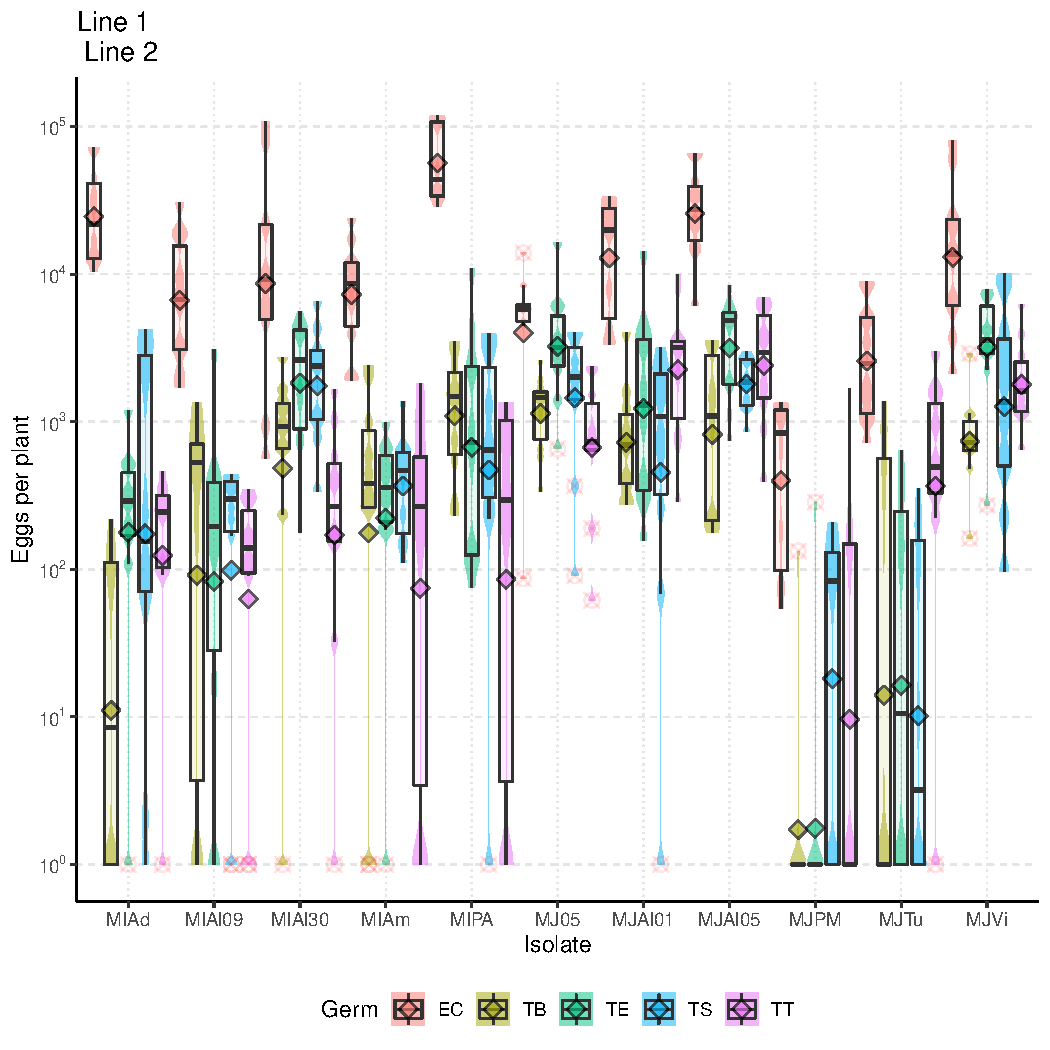
\includegraphics[width=\maxwidth]{figure/Plotssss-1} 

}	
			\end{adjustbox}
	\caption{Violin plots.}
	\label{fig:Figure01}
\end{figure}

\end{minipage}}

\end{frame}

\subsection{subsection b}

\begin{frame}
\frametitle{This is a frame with a table EC}
\scalebox{0.7}{\begin{minipage}{1.20\textwidth}

\begin{description}

\item[Item 1] texto de prueba 5
\item[Item 2] texto de prueba 6

\end{description}

\begin{figure}[ht]{}
	\captionsetup{width=\textwidth}
	\centering
	\begin{adjustbox}{width=\columnwidth, height=\height}
  \centering
  \resizebox{0.6\linewidth}{!}{

\begin{knitrout}
\definecolor{shadecolor}{rgb}{0.969, 0.969, 0.969}\color{fgcolor}
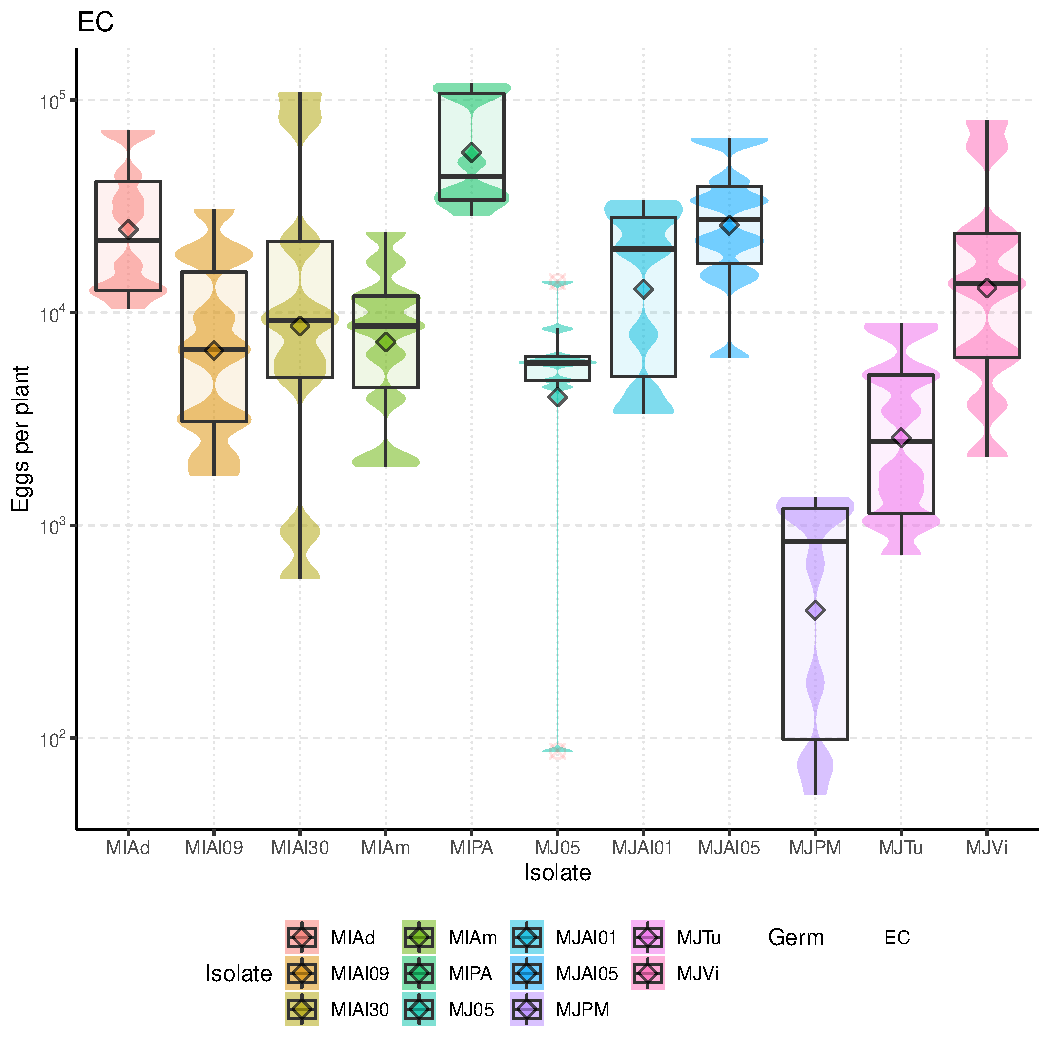
\includegraphics[width=\maxwidth]{figure/Plots_figure_individual_EC-1} 

\end{knitrout}
}
	\end{adjustbox}
	\caption{Density/Box plots Eggplant.}
	\label{fig:Figure02}
\end{figure}

\end{minipage}}

\end{frame}
\begin{frame}
\frametitle{This is a frame with a table TB}
\scalebox{0.7}{\begin{minipage}{1.20\textwidth}


\begin{columns}
\column{0.5\textwidth}
\begin{enumerate}[I]

\item texto de prueba 4


\item texto de prueba 4

\begin{itemize}
\item texto de prueba 5
\end{itemize}

\end{enumerate}
\column{0.5\textwidth}
\begin{enumerate}[I]

\item texto de prueba 4


\item texto de prueba 4

\begin{itemize}
\item texto de prueba 5
\end{itemize}

\end{enumerate}
\end{columns}

\begin{figure}[ht]{}
	\captionsetup{width=\textwidth}
	\centering	
	\begin{adjustbox}{width=\columnwidth, height=0.7\height}


\resizebox{0.8\linewidth}{!}{
\begin{knitrout}
\definecolor{shadecolor}{rgb}{0.969, 0.969, 0.969}\color{fgcolor}
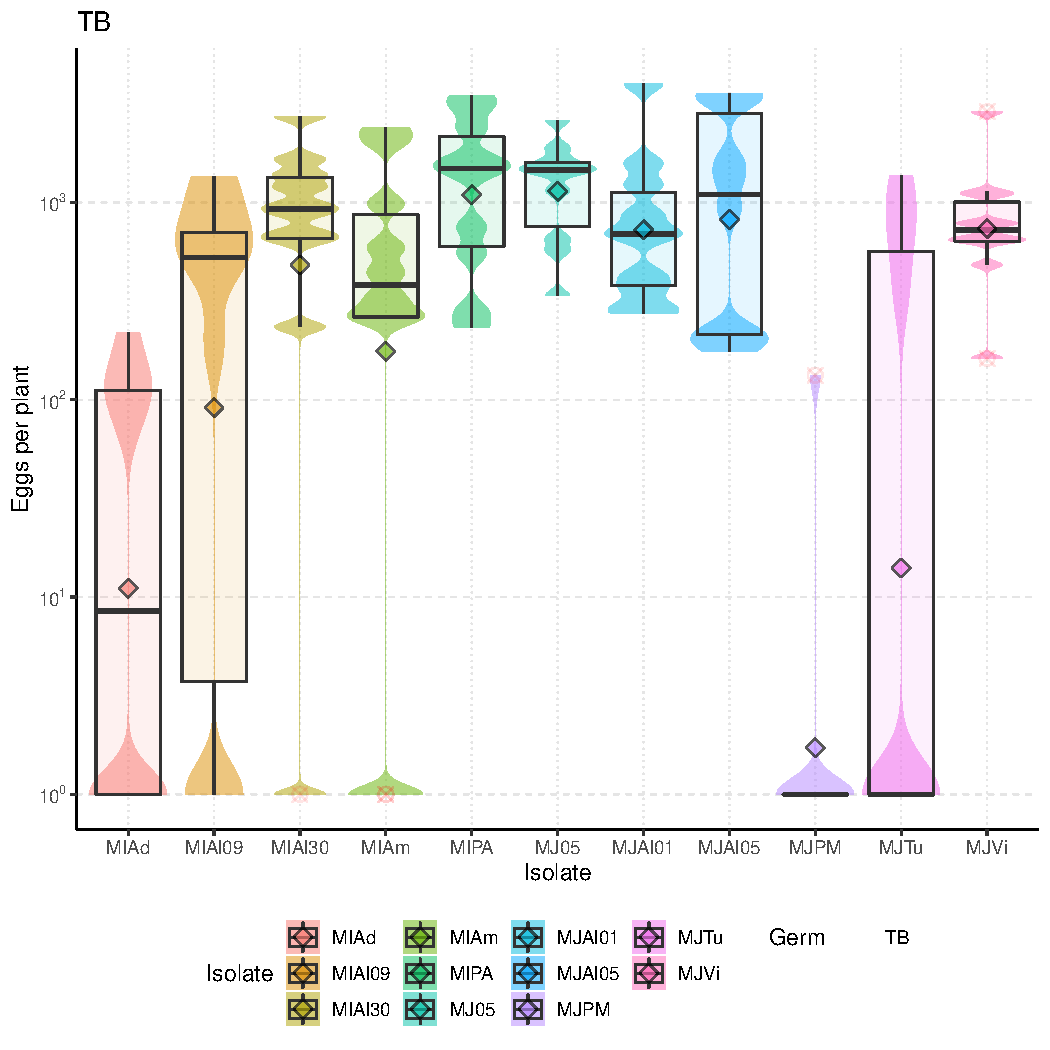
\includegraphics[width=\maxwidth]{figure/Plots_figure_individual_TB-1} 

\end{knitrout}
}
	\end{adjustbox}
	\caption{Density/Box plots Eggplant.}
	\label{fig:Figure03}
\end{figure}

\end{minipage}}

\end{frame}
\begin{frame}
\frametitle{This is a frame with a table TE}
\scalebox{0.7}{\begin{minipage}{1.20\textwidth}


\begin{columns}
\column{0.5\textwidth}
\begin{description}

\item[Item 1] texto de prueba 5
\item[Item 2] texto de prueba 6

\end{description}
\column{0.5\textwidth}
\begin{description}

\item[Item 1] texto de prueba 5
\item[Item 2] texto de prueba 6

\end{description}
\end{columns}


\begin{figure}[ht]{}
	\captionsetup{width=\textwidth}
	\centering	
	\begin{adjustbox}{width=\columnwidth, height=0.7\height}


\resizebox{0.8\linewidth}{!}{
\begin{knitrout}
\definecolor{shadecolor}{rgb}{0.969, 0.969, 0.969}\color{fgcolor}
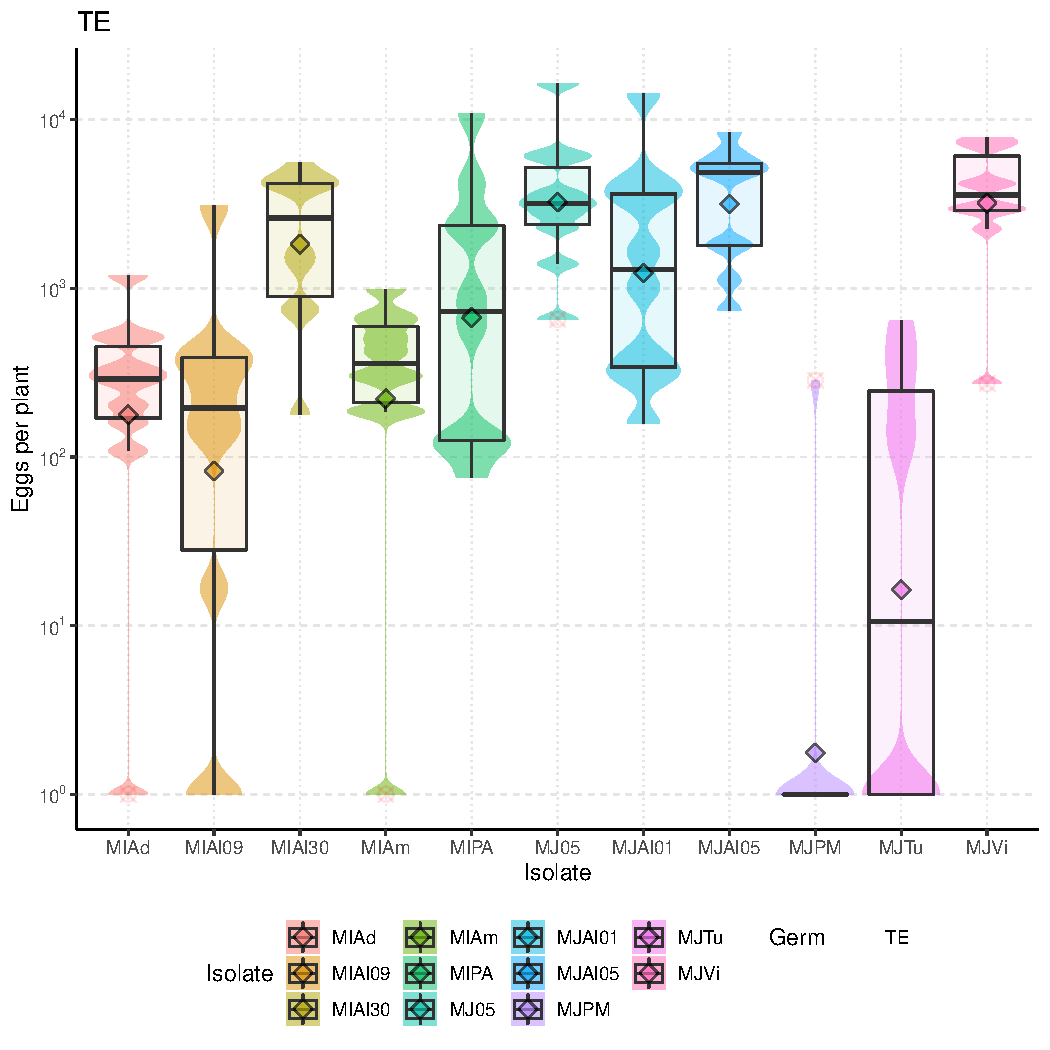
\includegraphics[width=\maxwidth]{figure/Plots_figure_individual_TE-1} 

\end{knitrout}
}
	\end{adjustbox}
	\caption{Density/Box plots Eggplant.}
	\label{fig:Figure02}
\end{figure}

\end{minipage}}

\end{frame}
\begin{frame}
\frametitle{This is a frame with a table TS}
\scalebox{0.7}{\begin{minipage}{1.20\textwidth}


\begin{block}{Block Title}
Lorem ipsum dolor sit amet, consectetur adipisicing elit, 
sed do eiusmod tempor incididunt ut labore et 
dolore magna aliqua.
\end{block}


\begin{figure}[ht]{}
	\captionsetup{width=\textwidth}
	\centering	
	\begin{adjustbox}{width=\columnwidth, height=0.7\height}


\resizebox{0.8\linewidth}{!}{
\begin{knitrout}
\definecolor{shadecolor}{rgb}{0.969, 0.969, 0.969}\color{fgcolor}
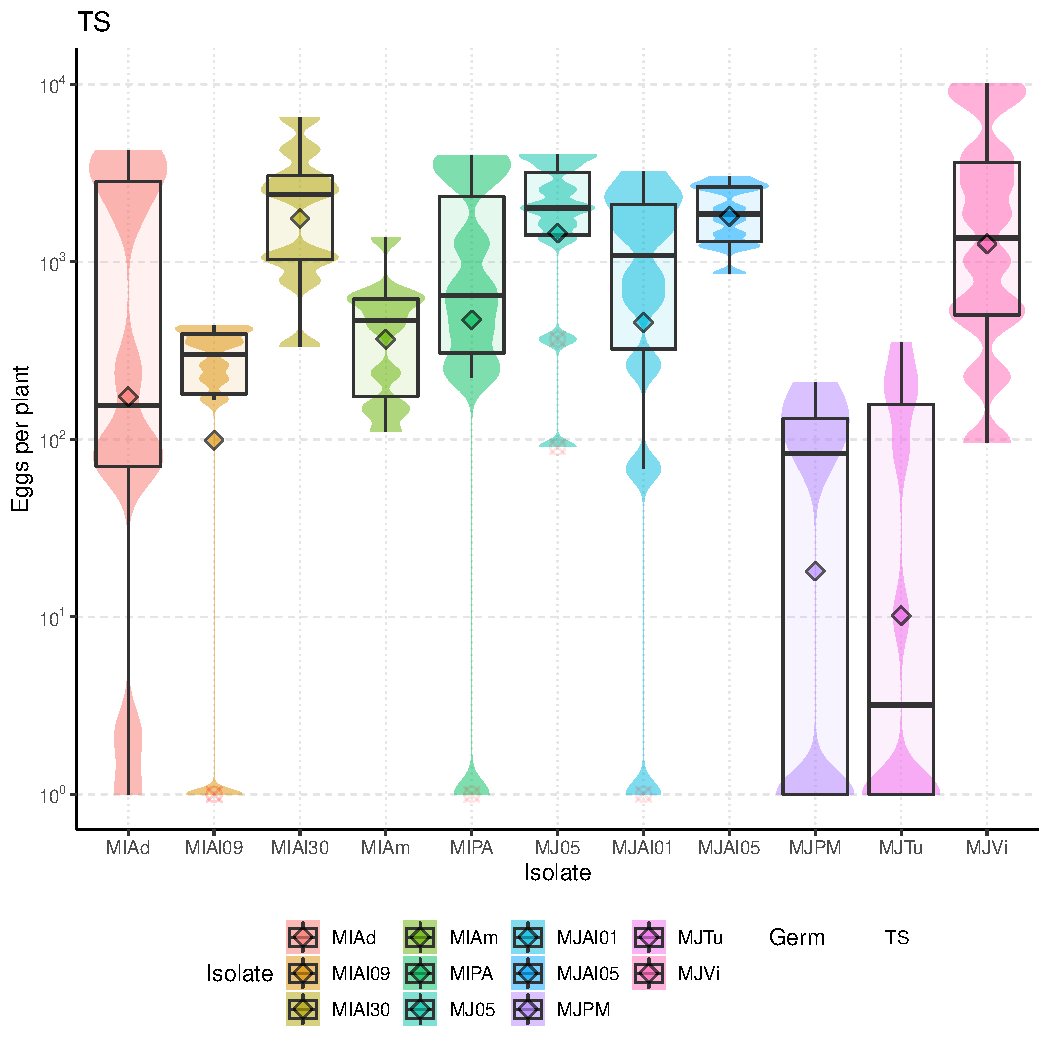
\includegraphics[width=\maxwidth]{figure/Plots_figure_individual_TS-1} 

\end{knitrout}
}
	\end{adjustbox}
	\caption{Density/Box plots Eggplant.}
	\label{fig:Figure02}
\end{figure}

\end{minipage}}

\end{frame}
\begin{frame}
\frametitle{This is a frame with a table TT}
\scalebox{0.7}{\begin{minipage}{1.20\textwidth}


\begin{alertblock}{Block Title}
Lorem ipsum dolor sit amet, consectetur adipisicing elit, 
sed do eiusmod tempor incididunt ut labore et 
dolore magna aliqua.
\end{alertblock}


\begin{figure}[ht]{}
	\captionsetup{width=\textwidth}
	\centering	
	\begin{adjustbox}{width=\columnwidth, height=0.7\height}


\resizebox{0.8\linewidth}{!}{
\begin{knitrout}
\definecolor{shadecolor}{rgb}{0.969, 0.969, 0.969}\color{fgcolor}
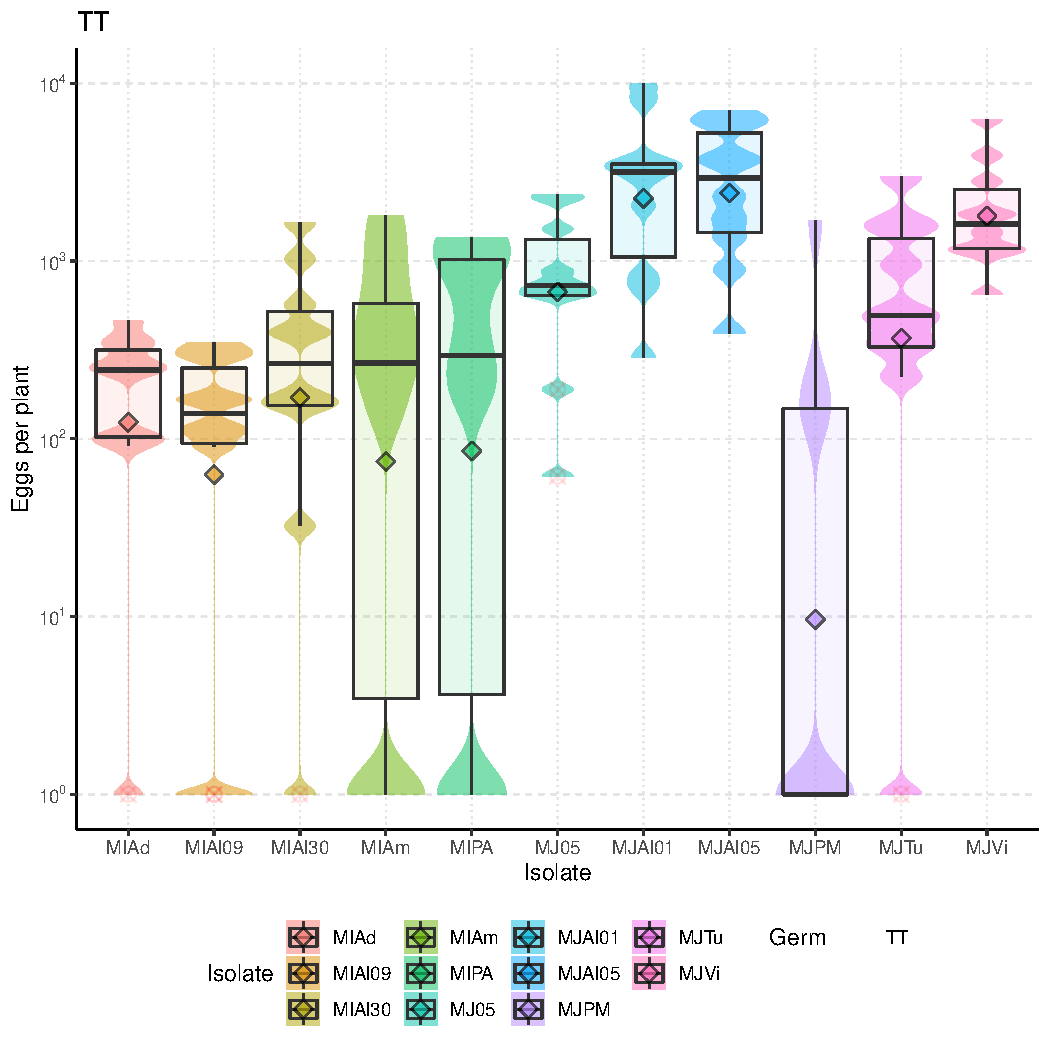
\includegraphics[width=\maxwidth]{figure/Plots_figure_individual_TT-1} 

\end{knitrout}
}
	\end{adjustbox}
	\caption{Density/Box plots Eggplant.}
	\label{fig:Figure02}
\end{figure}

\end{minipage}}

\end{frame}

\subsection{subsection c}

\begin{frame}

\frametitle{This is a frame with a table 10}
\scalebox{0.7}{\begin{minipage}{1.20\textwidth}


\begin{definition}
A prime number is a number that...
\end{definition}


\begin{figure}[ht]{}
	\captionsetup{width=\textwidth}


\centering
	\begin{adjustbox}{width=1\width, height=1\height}
\resizebox{0.7\linewidth}{!}{

\begin{knitrout}
\definecolor{shadecolor}{rgb}{0.969, 0.969, 0.969}\color{fgcolor}
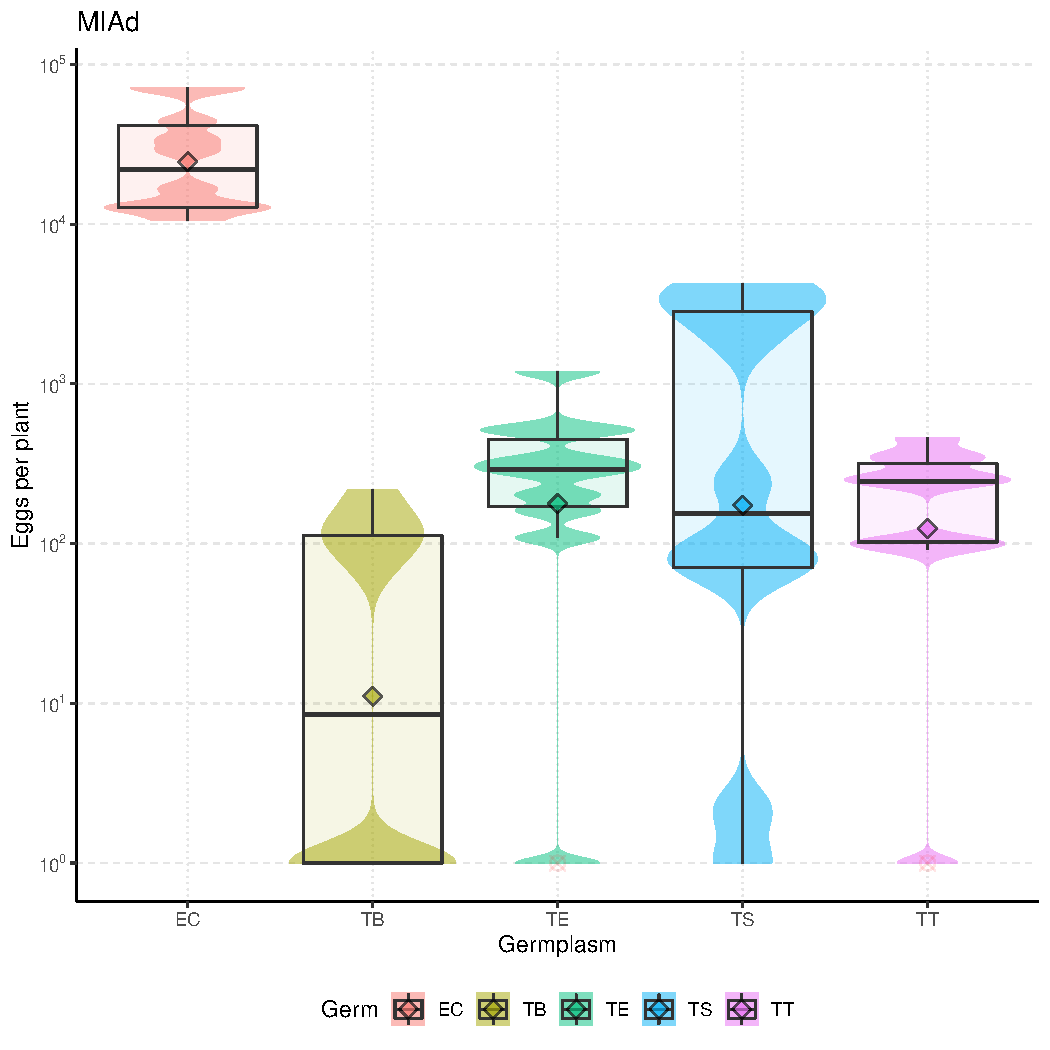
\includegraphics[width=\maxwidth]{figure/Plots_figure_individual_MIAd-1} 

\end{knitrout}
}
		\end{adjustbox}
			\caption{Density/Box plots Eggplant.}
	\label{fig:Figure033}
\end{figure}
		
	\end{minipage}}
	
		
\end{frame}



\begin{frame}[fragile]

\frametitle{This is a frame with a table 11}
\scalebox{0.7}{\begin{minipage}{1.20\textwidth}

\begin{columns}
\column{0.3\textwidth}
\begin{description}

\item[Item 1] Test5
  Test6
\item[Item 2] Test 7

\end{description}
\column{0.3\textwidth}
\begin{description}

\item[Item 1] Test 5
\item[Item 2] Test 6

\end{description}
\column{0.4\textwidth}
\begin{description}

\item[Item 1] \hyperlink{contents}{\beamerbutton{contents}}

\item[Item 2] \hyperlink{contents}{\beamerbutton{contents}}


\end{description}
\end{columns}



\begin{figure}[ht]{}
	\captionsetup{width=\textwidth}


\centering
	\begin{adjustbox}{width=1\width, height=1\height}
\resizebox{0.7\linewidth}{!}{

\begin{knitrout}
\definecolor{shadecolor}{rgb}{0.969, 0.969, 0.969}\color{fgcolor}
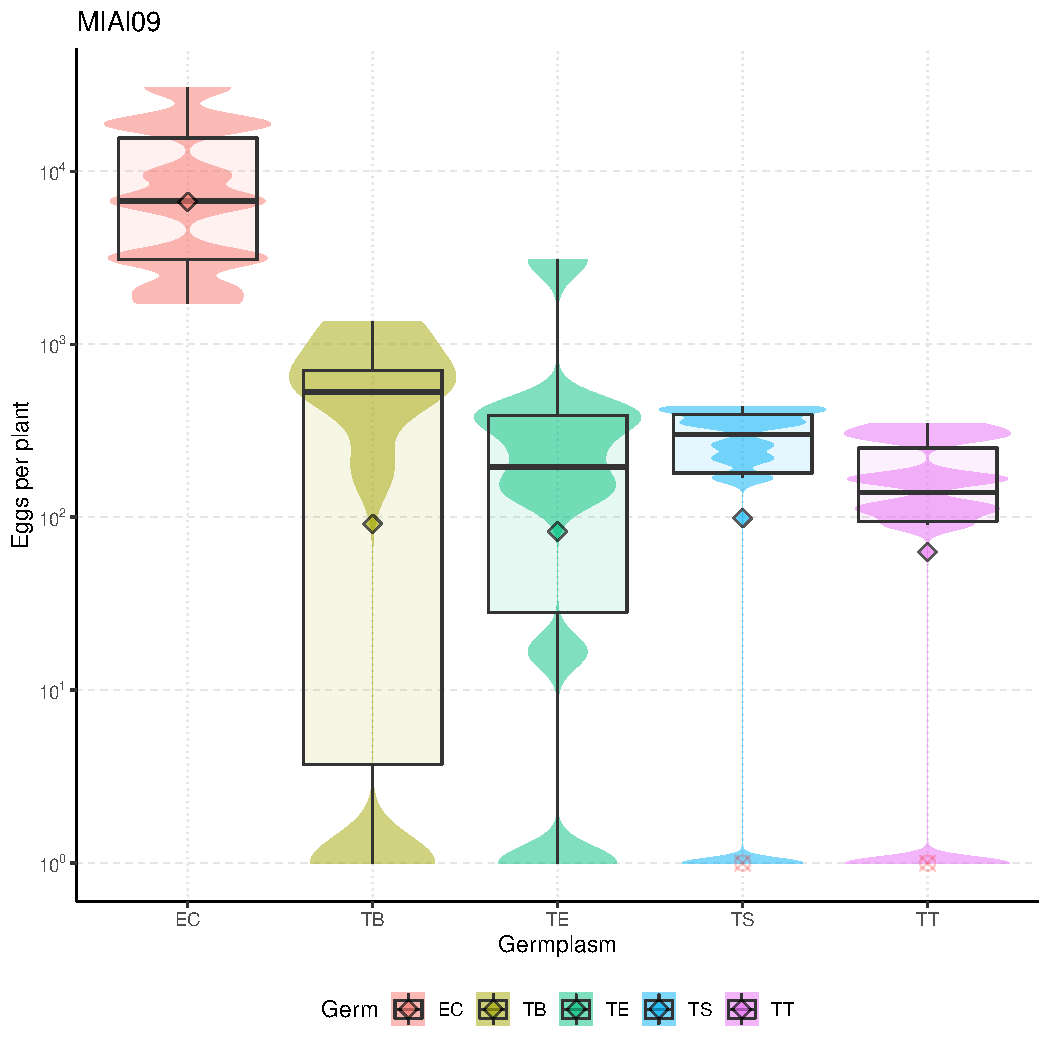
\includegraphics[width=\maxwidth]{figure/Plots_figure_individual_MIAl09-1} 

\end{knitrout}
}
		\end{adjustbox}
			\caption{Density/Box plots Eggplant.}
	\label{fig:Figure033}
\end{figure}
		
\end{minipage}}
		
		
	\end{frame}



\begin{frame}

\frametitle{This is a frame with a table 12}
\scalebox{0.7}{\begin{minipage}{1.20\textwidth}


\begin{columns}
\column{0.3\textwidth}
\begin{description}

\item[Item 1] Test5
\pause
  Test6
\pause
\item[Item 2] Test 7
\pause
\end{description}
\column{0.3\textwidth}
\begin{description}

\item[Item 1] Test 5
\pause
\item[Item 2] Test 6
\pause
\end{description}
\column{0.4\textwidth}
\begin{description}

\item[Item 1] \hyperlink{contents}{\beamerbutton{contents}}

\item[Item 2] \hyperlink{contents}{\beamerbutton{contents}}
\pause

\end{description}
\end{columns}


\begin{figure}[ht]{}
	\captionsetup{width=\textwidth}


\centering	
	\begin{adjustbox}{width=1\width, height=1\height}
\resizebox{0.7\linewidth}{!}{

\begin{knitrout}
\definecolor{shadecolor}{rgb}{0.969, 0.969, 0.969}\color{fgcolor}
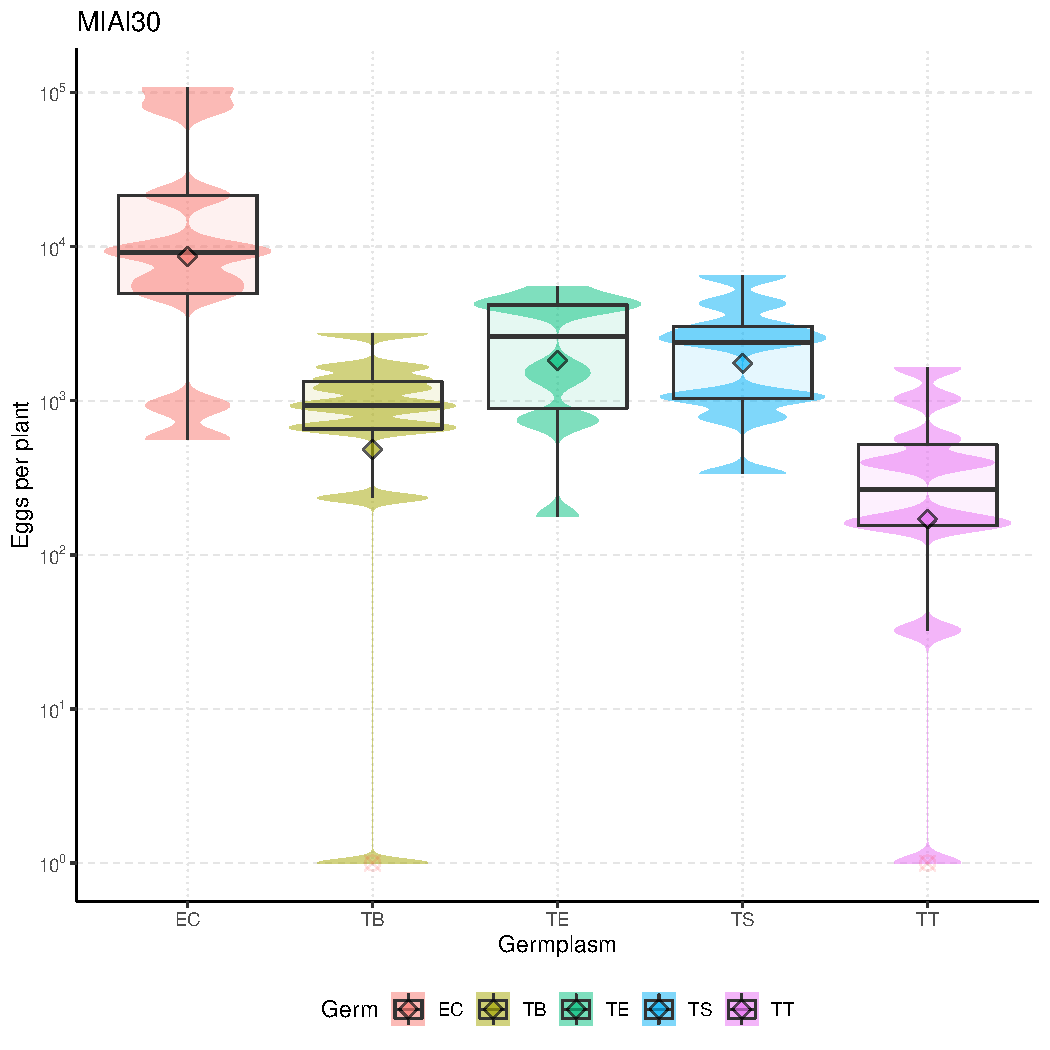
\includegraphics[width=\maxwidth]{figure/Plots_figure_individual_MIAl30-1} 

\end{knitrout}
}
		\end{adjustbox}
			\caption{Density/Box plots Eggplant.}
	\label{fig:Figure033}
\end{figure}
		
		
	\end{minipage}}
	
		
	\end{frame}



\begin{frame}

\frametitle{This is a frame with a table 13}
\scalebox{0.7}{\begin{minipage}{1.20\textwidth}


\begin{columns}
\column{0.3\textwidth}
\begin{description}

\item<1,2,3->[Item 1] Test5
\pause
  Test6
\pause
\item<2,4->[Item 2] Test 7
\pause
\end{description}
\column{0.3\textwidth}
\begin{description}

\item[Item 1] Test 5
\pause
\item[Item 2] Test 6
\pause
\end{description}
\column{0.4\textwidth}
\begin{description}

\item[Item 1] \hyperlink{contents}{\beamerbutton{contents}}

\item[Item 2] \hyperlink{contents}{\beamerbutton{contents}}
\pause

\end{description}
\end{columns}

\begin{figure}[ht]{}
	\captionsetup{width=\textwidth}


\centering	
			\begin{adjustbox}{width=1\width, height=1\height}
\resizebox{0.7\linewidth}{!}{

\begin{knitrout}
\definecolor{shadecolor}{rgb}{0.969, 0.969, 0.969}\color{fgcolor}
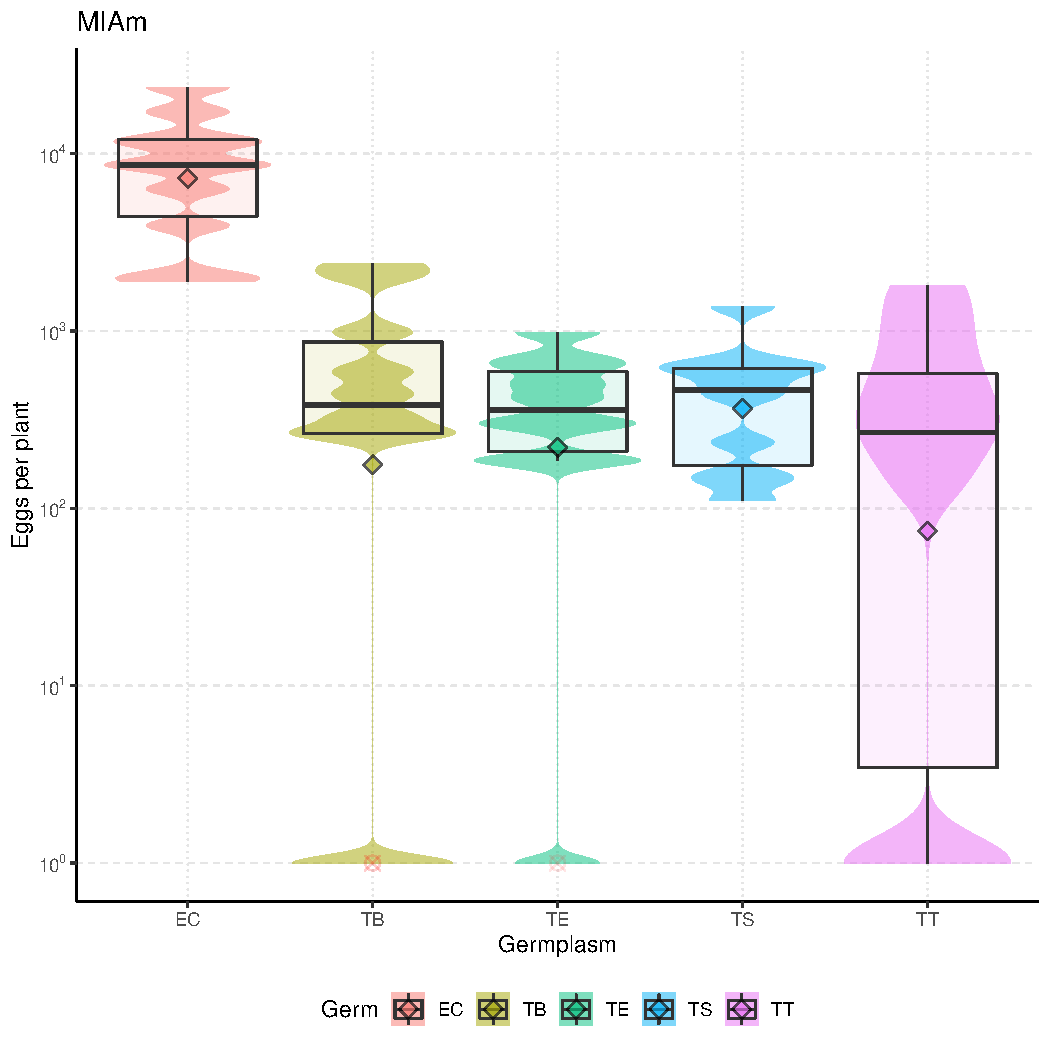
\includegraphics[width=\maxwidth]{figure/Plots_figure_individual_MIAm-1} 

\end{knitrout}
}
		\end{adjustbox}
			\caption{Density/Box plots Eggplant.}
	\label{fig:Figure033}
\end{figure}
		
	\end{minipage}}
	
		
	\end{frame}



\begin{frame}

\frametitle{This is a frame with a table 14}
\scalebox{0.7}{\begin{minipage}{1.20\textwidth}


\onslide<1->{First Line of Text}
 
\onslide<2->{Second Line of Text}
 
\onslide<3->{Third Line of Text}


\begin{figure}[ht]{}
	\captionsetup{width=\textwidth}


\centering	
		\begin{adjustbox}{width=1\width, height=1\height}
\resizebox{0.7\linewidth}{!}{

\begin{knitrout}
\definecolor{shadecolor}{rgb}{0.969, 0.969, 0.969}\color{fgcolor}
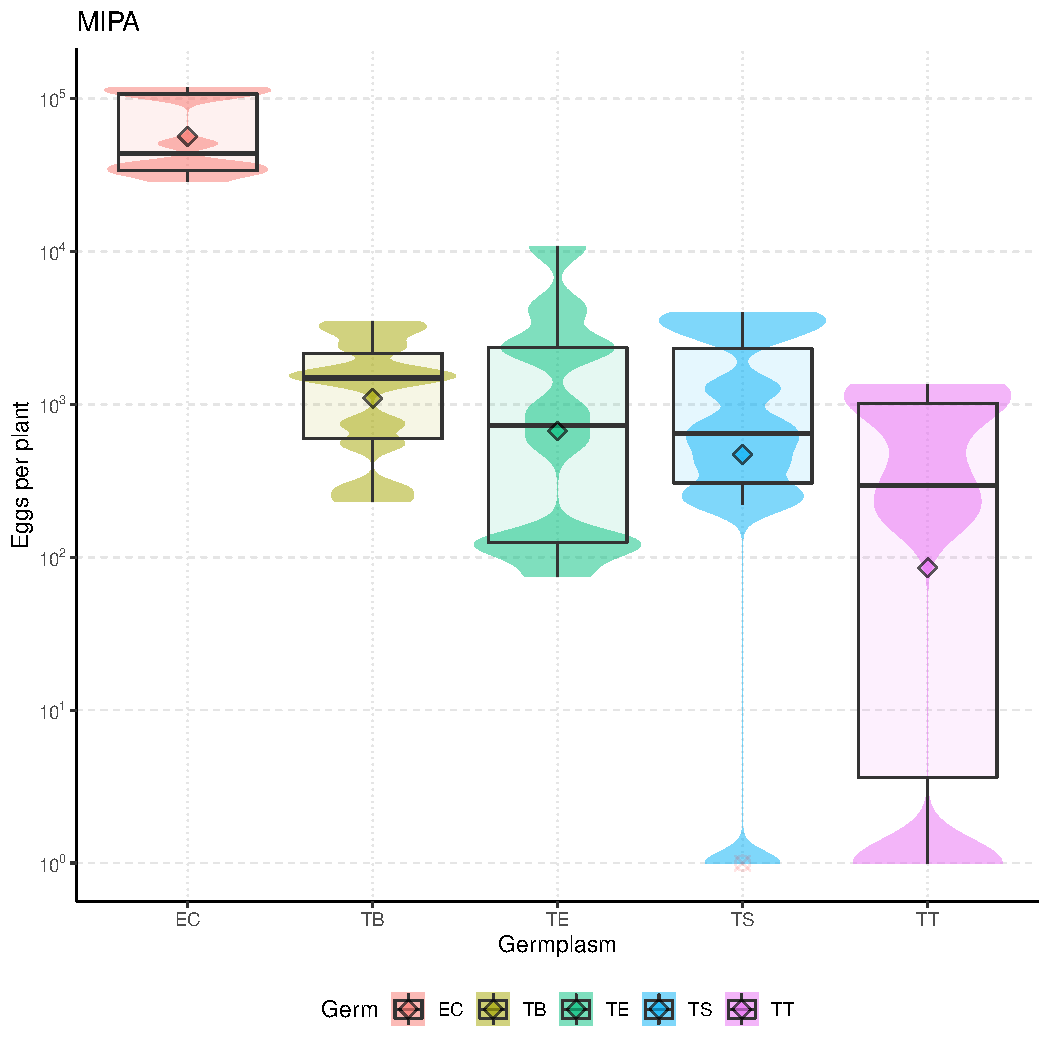
\includegraphics[width=\maxwidth]{figure/Plots_figure_individual_MIPa-1} 

\end{knitrout}
}
		\end{adjustbox}
			\caption{Density/Box plots Eggplant.}
	\label{fig:Figure033}
\end{figure}
		
		
	\end{minipage}}
	
		
	\end{frame}



\begin{frame}

\frametitle{This is a frame with a table 15}
\scalebox{0.7}{\begin{minipage}{1.20\textwidth}


\only<1>{First Line of Text}
 
\only<2>{Second Line of Text}
 
\only<3>{Third Line of Text}


\begin{figure}[ht]{}
	\captionsetup{width=\textwidth}


\centering	
		\begin{adjustbox}{width=1\width, height=1\height}
\resizebox{0.7\linewidth}{!}{

\begin{knitrout}
\definecolor{shadecolor}{rgb}{0.969, 0.969, 0.969}\color{fgcolor}
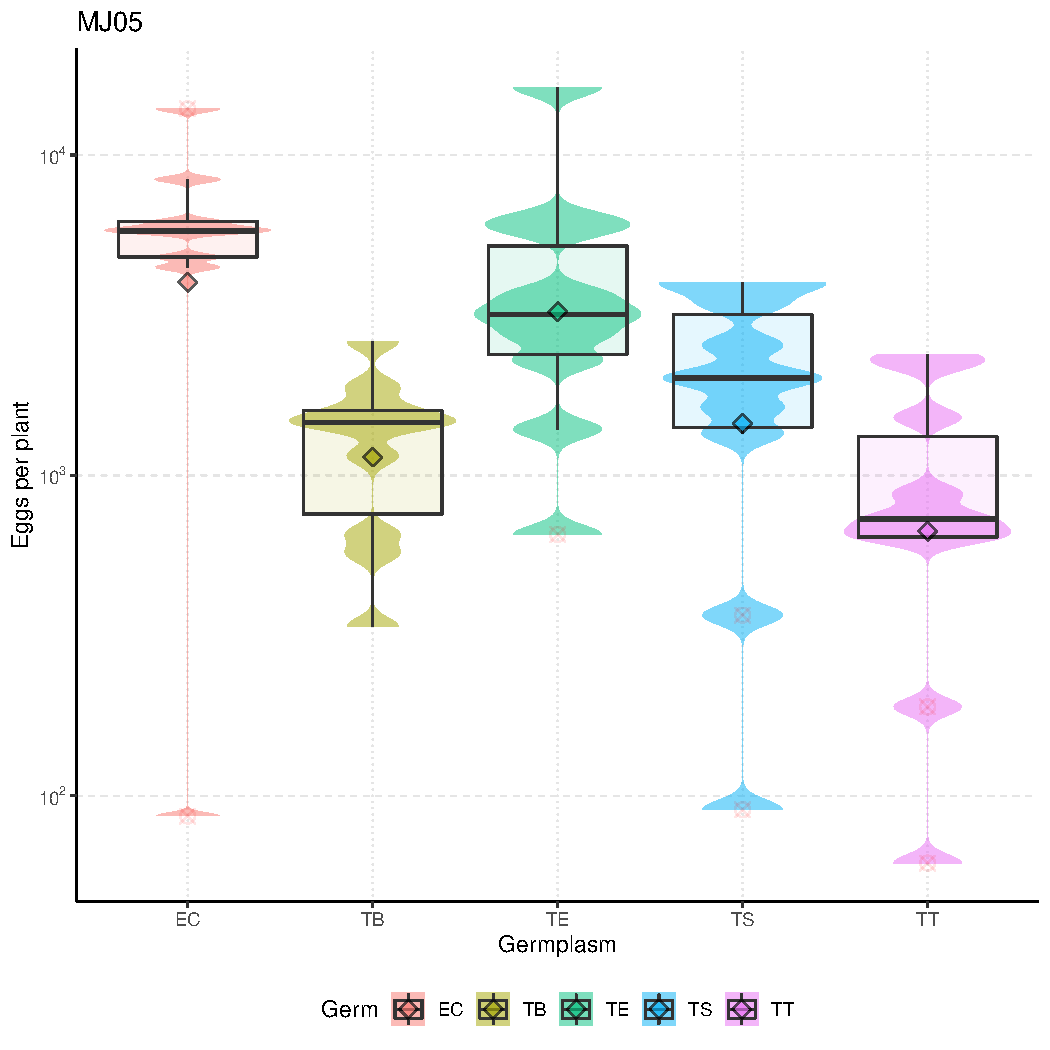
\includegraphics[width=\maxwidth]{figure/Plots_figure_individual_MJ05-1} 

\end{knitrout}
}
		\end{adjustbox}
			\caption{Density/Box plots Eggplant.}
	\label{fig:Figure033}
\end{figure}
		
		
	\end{minipage}}
	
		
	\end{frame}



\begin{frame}

\frametitle{This is a frame with a table 16}
\scalebox{0.7}{\begin{minipage}{1.20\textwidth}


\usecolortheme{fly}
erthrtyj+

yuil

\begin{figure}[ht]{}
	\captionsetup{width=\textwidth}


\centering	
		\begin{adjustbox}{width=1\width, height=1\height}
\resizebox{0.7\linewidth}{!}{

\begin{knitrout}
\definecolor{shadecolor}{rgb}{0.969, 0.969, 0.969}\color{fgcolor}
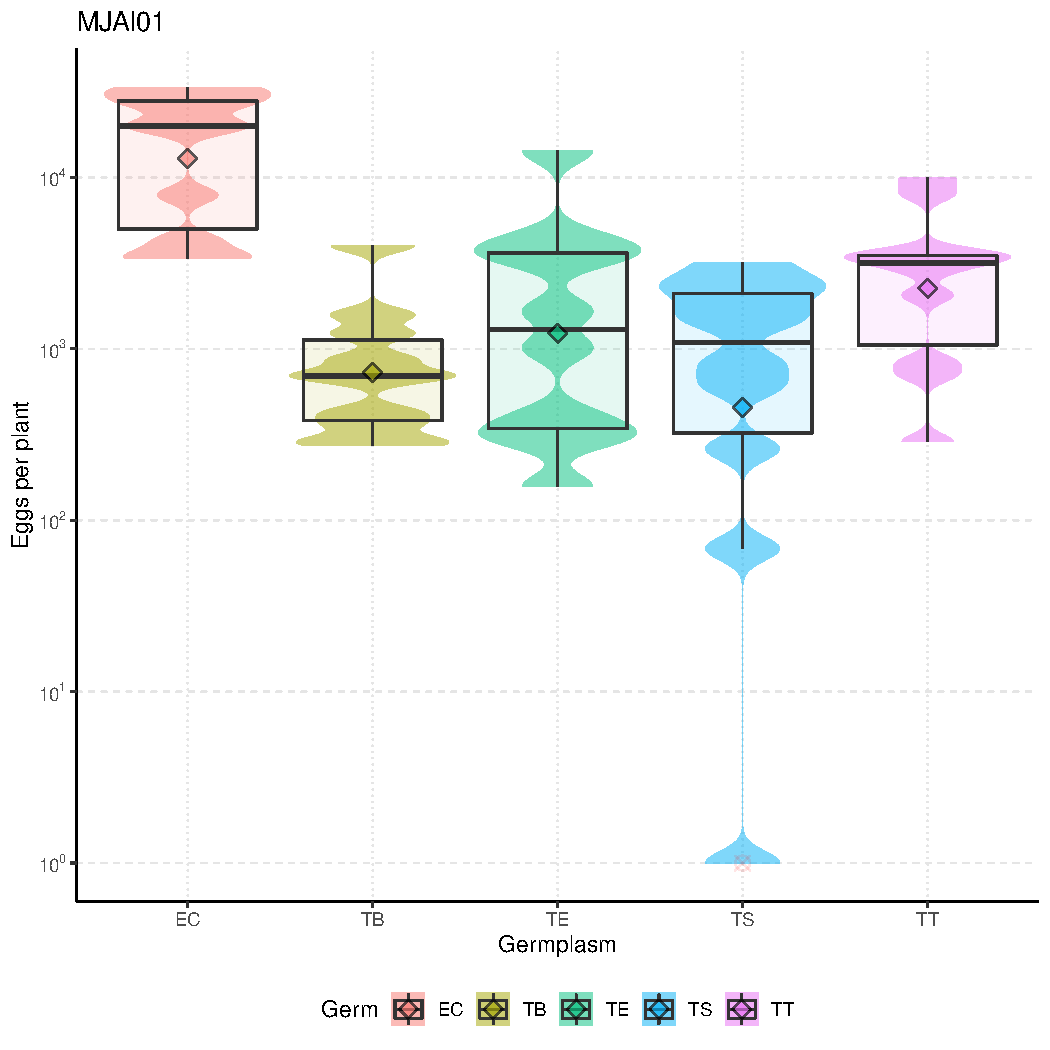
\includegraphics[width=\maxwidth]{figure/Plots_figure_individual_MJAl01-1} 

\end{knitrout}
}
		\end{adjustbox}
			\caption{Density/Box plots Eggplant.}
	\label{fig:Figure033}
\end{figure}
		
		
	\end{minipage}}
	
	\end{frame}



\begin{frame}

\frametitle{This is a frame with a table 17}
\scalebox{0.7}{\begin{minipage}{1.20\textwidth}


texto de prueba 17


\begin{figure}[ht]{}
	\captionsetup{width=\textwidth}


\centering			
		\begin{adjustbox}{width=1\width, height=1\height}
\resizebox{0.7\linewidth}{!}{

\begin{knitrout}
\definecolor{shadecolor}{rgb}{0.969, 0.969, 0.969}\color{fgcolor}
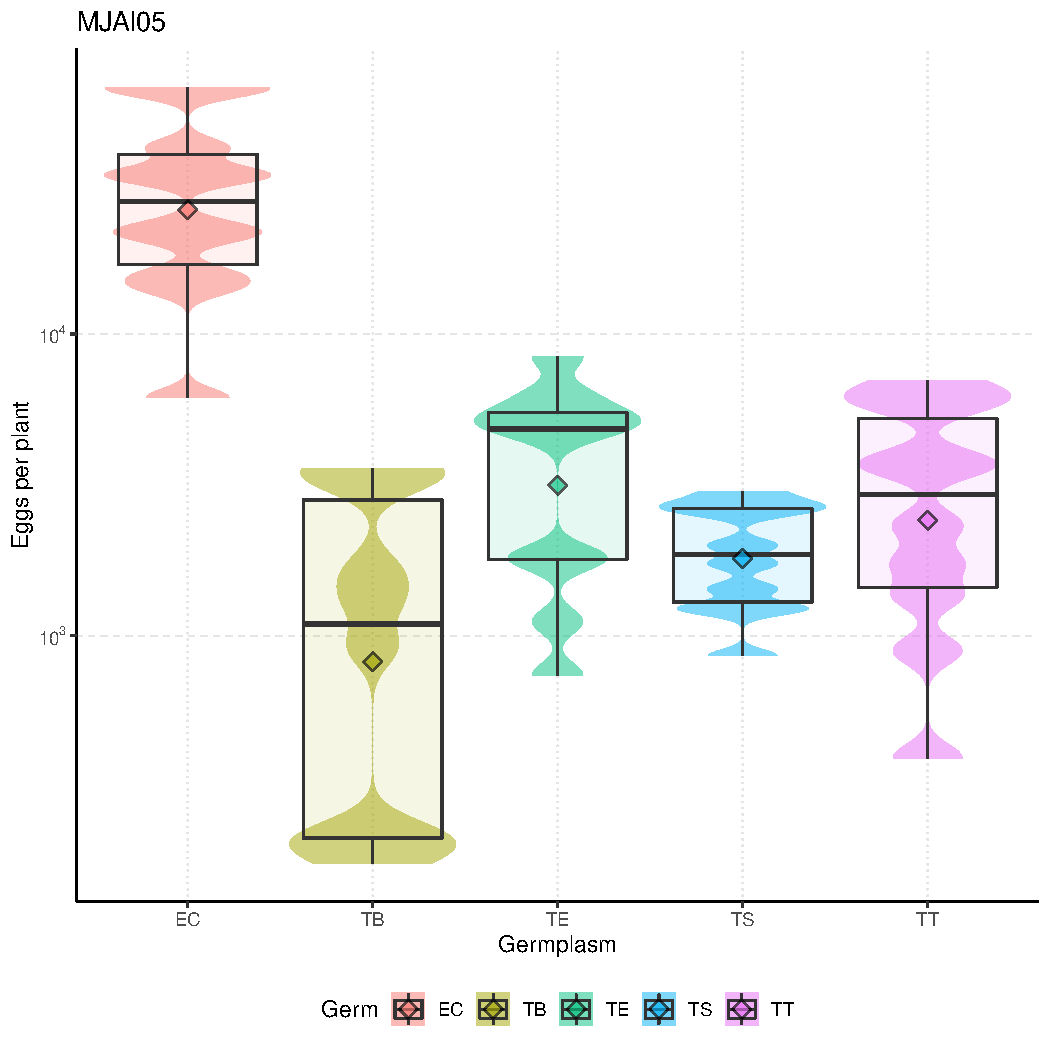
\includegraphics[width=\maxwidth]{figure/Plots_figure_individual_MJAl05-1} 

\end{knitrout}
}
		\end{adjustbox}
			\caption{Density/Box plots Eggplant.}
	\label{fig:Figure033}
\end{figure}
		
	\end{minipage}}
	
		
	\end{frame}



\begin{frame}

\frametitle{This is a frame with a table 18}
\scalebox{0.7}{\begin{minipage}{1.20\textwidth}


texto de prueba 18


\begin{figure}[ht]{}
	\captionsetup{width=\textwidth}


\centering	
		\begin{adjustbox}{width=1\width, height=1\height}
\resizebox{0.7\linewidth}{!}{

\begin{knitrout}
\definecolor{shadecolor}{rgb}{0.969, 0.969, 0.969}\color{fgcolor}
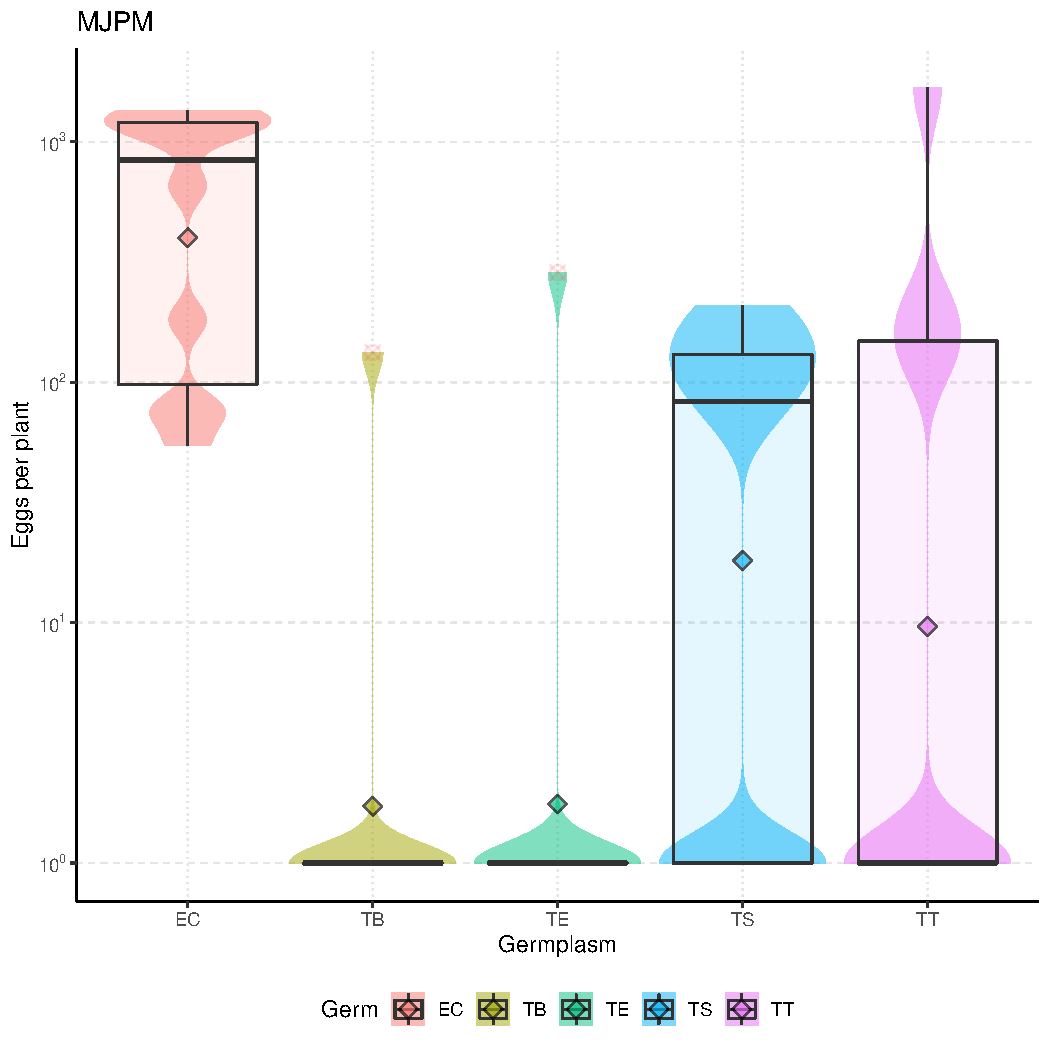
\includegraphics[width=\maxwidth]{figure/Plots_figure_individual_MJPM-1} 

\end{knitrout}
}
		\end{adjustbox}
			\caption{Density/Box plots Eggplant.}
	\label{fig:Figure033}
\end{figure}
		
		\end{minipage}}

		
\end{frame}



\begin{frame}

\frametitle{This is a frame with a table 19}
\scalebox{0.7}{\begin{minipage}{1.20\textwidth}


texto de prueba 19


\begin{figure}[ht]{}
	\captionsetup{width=\textwidth}


\centering
		\begin{adjustbox}{width=1\width, height=1\height}
\resizebox{0.7\linewidth}{!}{

\begin{knitrout}
\definecolor{shadecolor}{rgb}{0.969, 0.969, 0.969}\color{fgcolor}
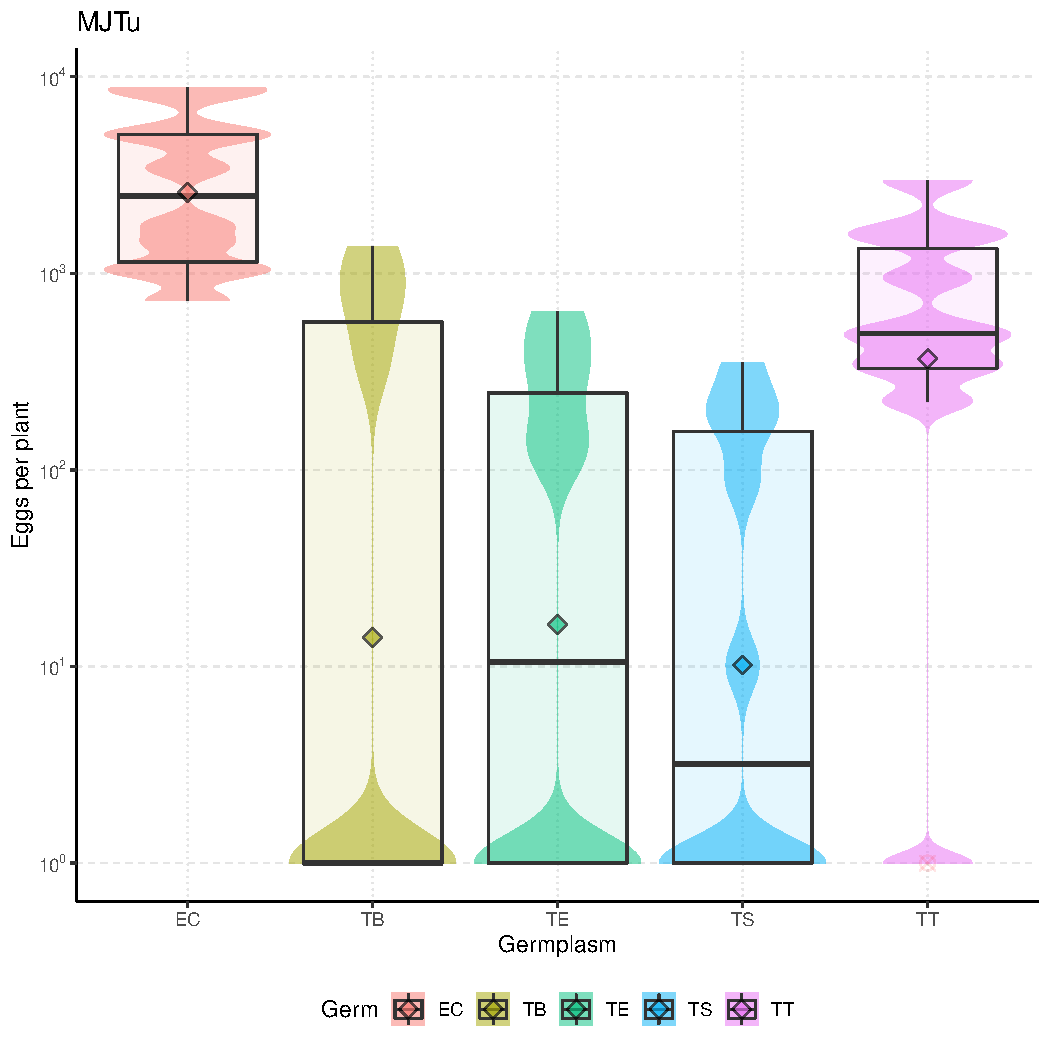
\includegraphics[width=\maxwidth]{figure/Plots_figure_individual_MJTu-1} 

\end{knitrout}
}
		\end{adjustbox}
			\caption{Density/Box plots Eggplant.}
	\label{fig:Figure033}
\end{figure}
		
		\end{minipage}}

		
\end{frame}



\begin{frame}

\frametitle{This is a frame with a table 20}
\scalebox{0.7}{\begin{minipage}{1.20\textwidth}


\begin{columns}
\column{0.5\textwidth}
text 20
\column{0.5\textwidth}
text 21
\end{columns}

\begin{figure}[ht]{}
	\captionsetup{width=\textwidth}


\centering
		\begin{adjustbox}{width=1\width, height=1\height}
\resizebox{0.7\linewidth}{!}{

\begin{knitrout}
\definecolor{shadecolor}{rgb}{0.969, 0.969, 0.969}\color{fgcolor}
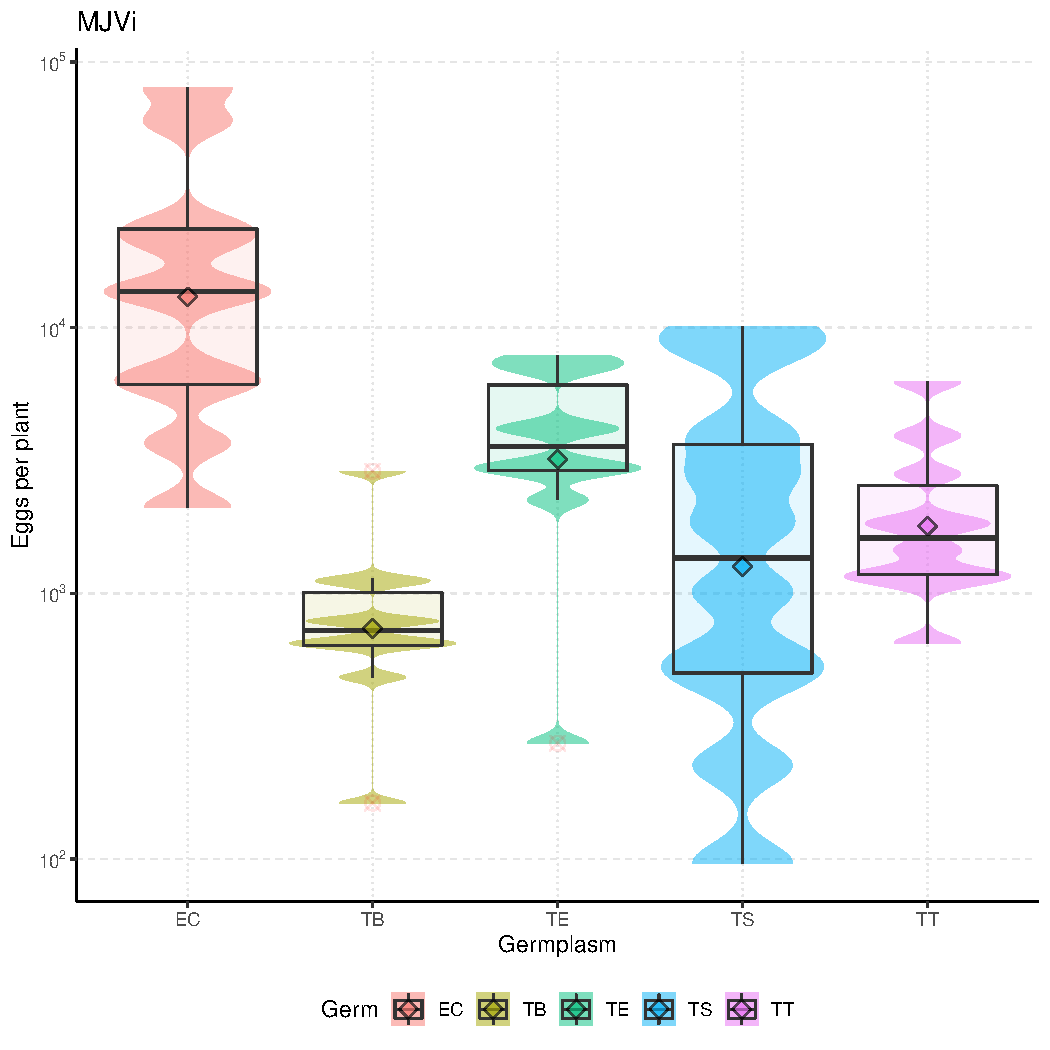
\includegraphics[width=\maxwidth]{figure/Plots_figure_individual_MJVi-1} 

\end{knitrout}
}
		\end{adjustbox}
		
		
		
		


	\caption{Density/Box plots Eggplant.}
	\label{fig:Figure033}
\end{figure}

\end{minipage}}


\end{frame}

\begin{frame}[fragile]
\frametitle{Including Code}
\scalebox{0.7}{\begin{minipage}{1.20\textwidth}

\begin{semiverbatim}
\\begin\{frame\}
\\frametitle\{Outline\}
\\tableofcontents
\\end\{frame\}
\end{semiverbatim}

\end{minipage}}

\end{frame}

\begin{frame}
\frametitle{buttons}
\scalebox{0.7}{\begin{minipage}{1.20\textwidth}


\hyperlink{contents}{\beamerbutton{contents page}}

\end{minipage}}

\end{frame}

\end{document}
